The electrodes and contact pads of photoconductive antennas are designed mainly to provide bias and current extraction. In practice they strongly affect the antenna’s performance. At low THz frequencies (typically \num{50} - \num{100}\,\si{\giga \hertz}), the relatively large metal pads and finite feeding strips act as resonant
structures. They couple efficiently to long-wavelength components of the THz pulse, giving rise to strong
surface currents and standing waves. These resonances dominate the measured time-domain traces, where they appear as long-lasting oscillations following the main THz pulse. In the frequency domain, they manifest as sharp spectral peaks that obscure higher-frequency information of interest.

\subsection{Fourier Transformation as Analysis Tool}

The effect of resonances can be analyzed by transforming time-domain THz signals into the frequency domain
via Fourier transformation. The Fourier transform of a real-valued time-domain pulse is a complex-valued frequency-domain spectrum. Analytically this yields \cite{MathematicalMethodsPhysics} 
\begin{equation}
    \mathcal{F}\left\{
        E_{Thz}(t) 
    \right\} = \beta \int_{-\infty}^{+\infty} E_{THz}(t)e^{i\omega t} = E_{THz}(\omega),
\end{equation}

where $\beta$ is a normalization factor that may differ depending on the field of study and the algorithm used. For discrete data, the analytical Fourier transform cannot be used. In this work, the fast Fourier transform (FFT) is used to obtain the THz spectrum. The FFT is an efficient implementation of the discrete Fourier transformation (DFT). The DFT maps a finite number of measurements $x(n)$ into the frequency domain. Many DFT properties are similar to the analog Fourier transformation. The DFT is defined as \cite{raoFastFourierTransform2010}
\begin{equation}
    X^F(k) = \beta \sum_{n = 0}^{N - 1}x(n)e^{\frac{-i2\pi k n}{N}}, \qquad k = 0, 1, ..., N-1, \qquad n = 0, 1, ..., N-1,
\end{equation}

where $x(n)$ denotes a uniformly sampled sequence and $X^F(k)$ is the $k$-th DFT coefficient. Figure \ref{fig:FFT} exemplarily  shows 
low-frequency oscillations in the time-domain translating into sharp peaks in the frequency-domain. A more non-resonant and broadband behavior is desired. 


\begin{figure}[!]
    \centering
    \begin{minipage}{\textwidth} 
        \centering
        \begin{subfigure}[t]{0.48\textwidth}
            \centering
            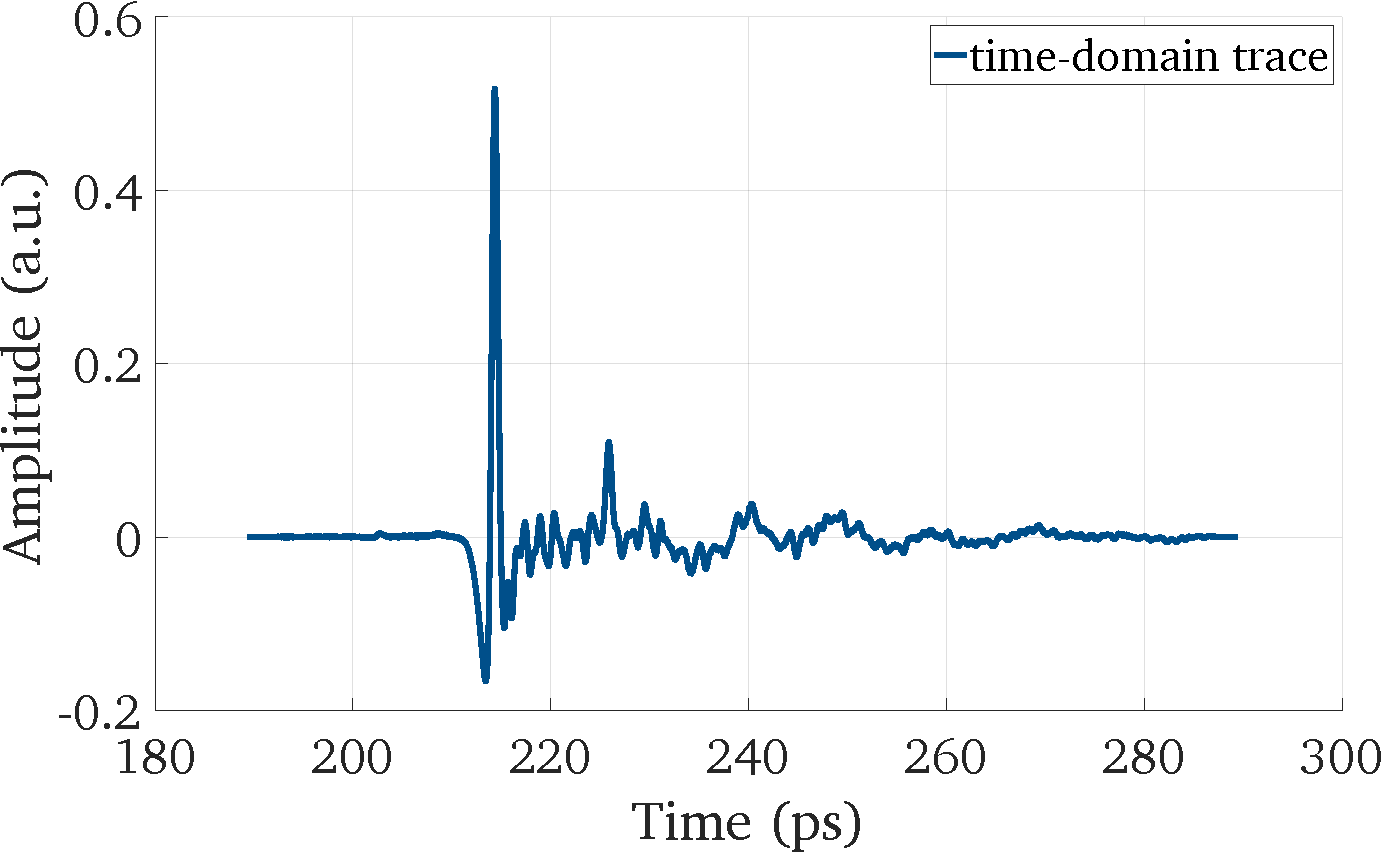
\includegraphics[height=0.235\textheight]{figures/FFT_time.pdf}
            \caption{\centering}
            \label{fgdhsjk}
        \end{subfigure}
        \hfill
        \begin{subfigure}[t]{0.48\textwidth}
            \centering
            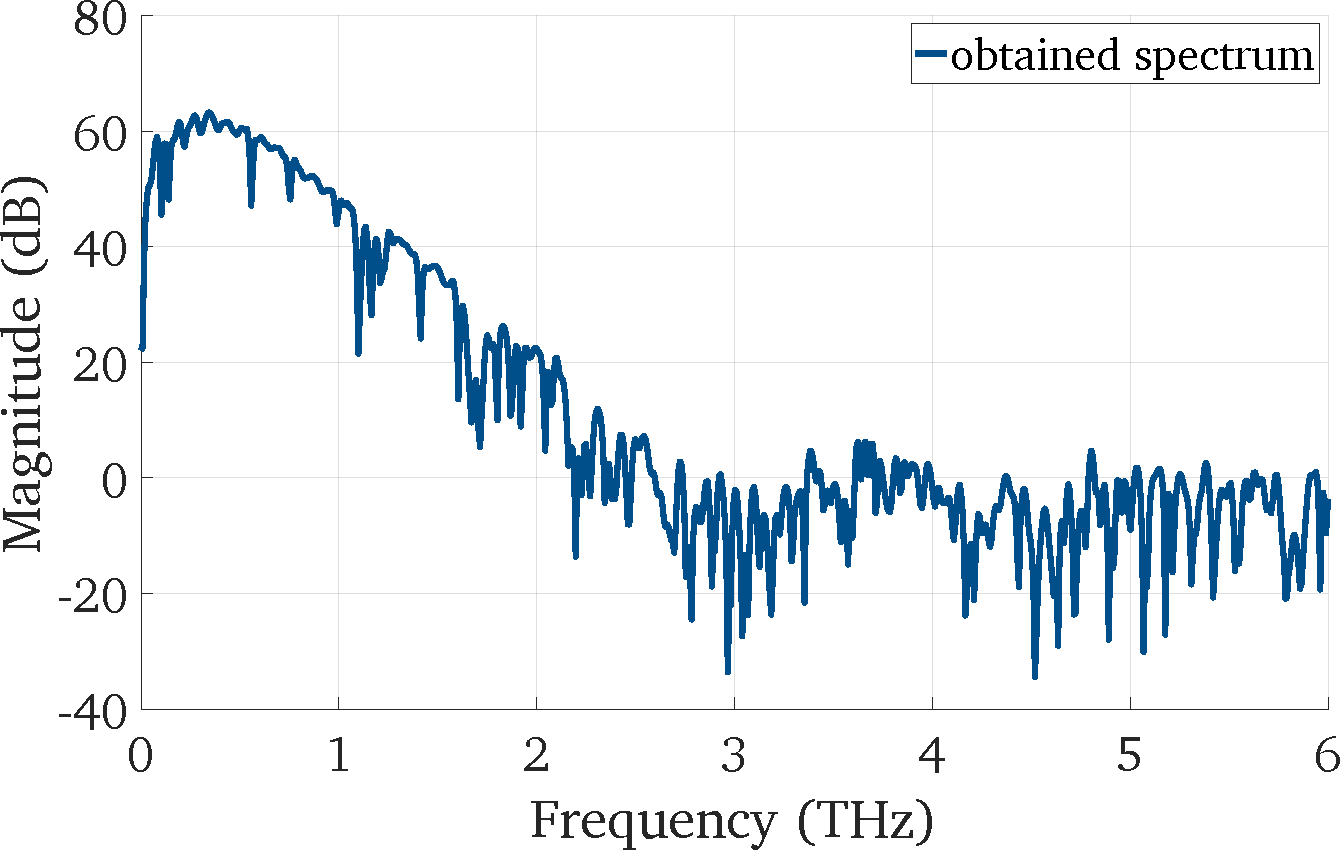
\includegraphics[height=0.235\textheight]{figures/FFT_spectrum.pdf}
            \caption{\centering}
            \label{ghjkl}
        \end{subfigure}
        \caption{Exemplary FFT of a time-domain THz pulse. (a) Time-domain data. Time-harmonic oscillations are observed (b) FFT spectrum. Sharp spectral features are observed.}
        \label{fig:FFT}
    \end{minipage}
\end{figure}

\subsection{Low Frequency Pad Resonances}

The origin of these effects can be understood by considering the scale of the antenna geometry. At low frequencies (wavelengths of $\lambda \sim 3\,$\,\si{\milli \meter} to $6\,$\,\si{\milli \meter}), the antenna electrodes are much smaller
than $\lambda$. Electromagnetic waves couple most efficiently to resonant structures. Resonant in this context means a structure with a width that is a multiple of the EM-waves wavelength. Typically those multiples are $\frac{1}{4}$, $\frac{1}{2}$ or \num{1}. This results in the THz waves coupling to the antenna's pads rather than the electrodes at low frequencies. The large pads result in large surface currents, turning them into unwanted resonators. The result is a pronounced low-frequency
response that does not necessarily contain useful THz information but dominates the measured signal.

\subsection{Low Frequency Time-Domain Harmonics}

In addition to pad resonances, standing waves form along the finite feeding strips of the antenna at lower frequencies ($\nu < 500$ \si{\giga \hertz}). These standing waves generate periodic oscillations in the time-domain signal, separated by $\Delta t \approx 20$\,\si{\pico \s}, corresponding to resonance frequencies around \num{50}\,\si{\giga \hertz}. Especially when investigating materials with high refractive indices, these time-harmonic oscillations can make measurements extremely challenging. Considering a very simplified case with normal incidence and where there is no distinction between the polarization of two materials, Fresnel's equations tell us that the reflectance $R$ becomes 
\begin{equation}
    R = \left| \frac{n_1 - n_2}{n_1 + n_2} \right|^2.
\end{equation}
A material with a high refractive index generally causes more reflections \cite{gallegosRefractiveIndex2025}. The actual THz signal may be hard to distinguish from the resonances caused by the standing wave propagation.

% Another unwanted effect at lower frequencies ($\nu < 500$ \si{\giga \hertz}) are resonant harmonics that are observable in the measured THz field. Reflections of non-radiative frequencies within the antenna's finite length feeding strip produce standing waves spaced apart by $\sim$\num{50} \si{\giga \hertz} with an effective wavelength equal to the strip's length. The resonant standing waves exhibit different propagation speeds compared to the emitted THz pulse. The dispersion causes undesired time-harmonic oscillations following the original THz pulse. Especially when investigating materials with high refractive indices, these time-harmonic oscillations can make measurements extremely challenging. Considering a very simplified case with normal incidence and where there is no distinction between the polarization of two materials, Fresnel's equations tell us that the reflectance $R$ becomes 
% \begin{equation}
%     R = \left| \frac{n_1 - n_2}{n_1 + n_2} \right|^2.
% \end{equation}
% A material with a high refractive index generally causes more reflections \cite{gallegosRefractiveIndex2025}. The actual THz signal may be hard to distinguish from the resonances caused by the standing wave propagation. 

% \begin{figure}[ht]
%   \centering
%     \centering
%     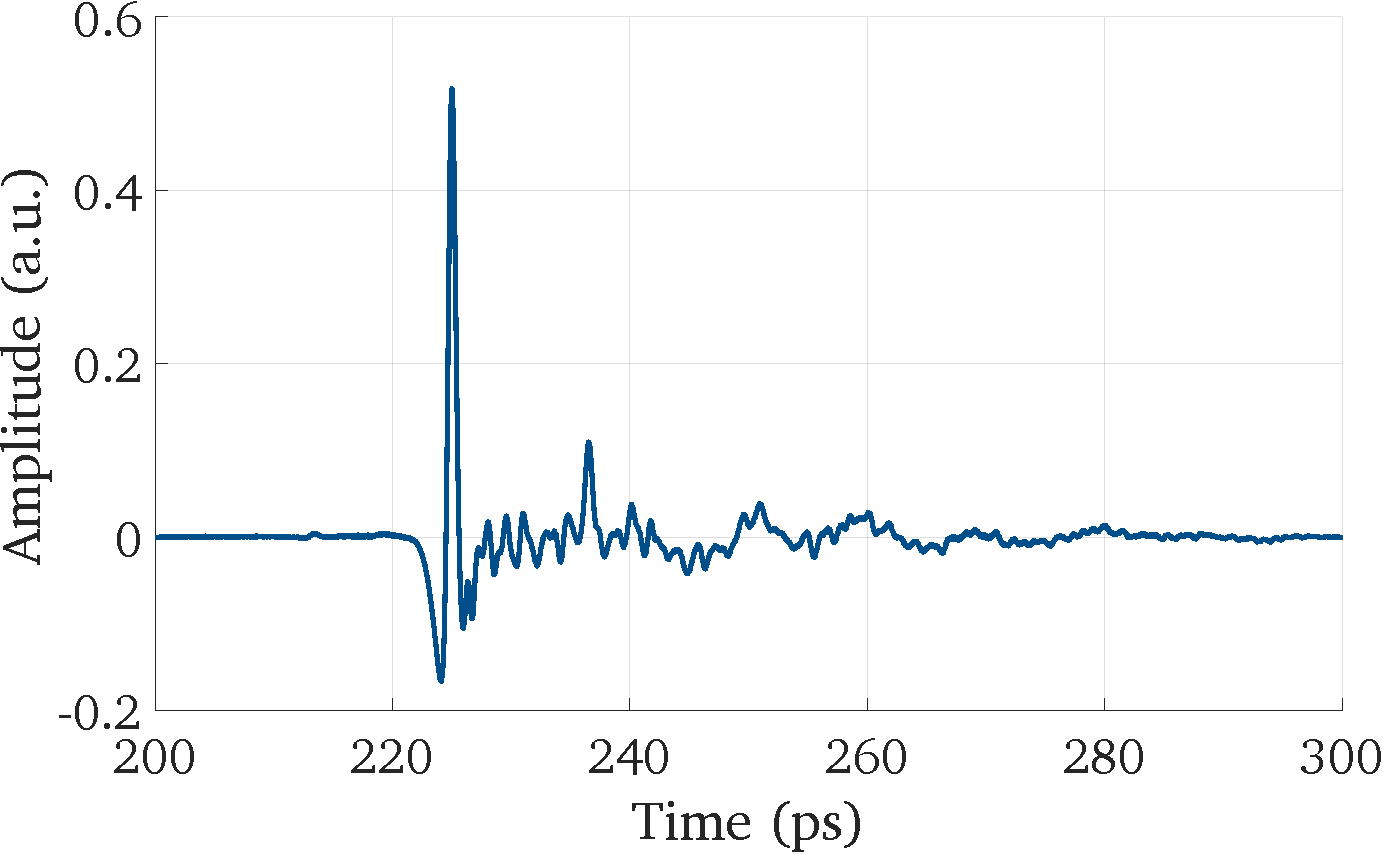
\includegraphics[width=0.6\linewidth]{figures/ringing_schem.pdf}
%     \caption{A THz pulse is observed, followed by distinct time-domain harmonics appearing after the main pulse. The first noticeable peak resulting from standing waves occurs at approx. \num{240} \si{\pico \s}. Subsequent peaks appear every \num{10} \si{\pico \s}, resulting in an oscillation period $T \approx 20$ \si{\pico \s}. This corresponds to a resonance in the spectrum at $f \approx 50$ \si{\giga \hertz}, caused by standing waves in the antenna Structure.} 
%     \label{fig:ringing}
% \end{figure}

\subsection{Motivation for Inclusion of Resistive Feeds}

The presence of pad-induced resonances fundamentally and standing wave oscillations in the antenna feed limits PCA performance in THz-TDS. Intrinsic performance limitations such as RC roll-off and carrier lifetime determine the high-frequency cutoff. These performance limiting factors are accounted for in the derivation of the spectrum and are well studied. In practice the low-frequency resonances are equally detrimental, because they prevent the extraction of clean broadband spectra that would be expected with the derivation of the spectra so far. The central idea of this thesis is to introduce resistive NiCr segments into the feeding lines (or Dipole arms in I-shaped Dipoles) of the antennas. These resistive sections act as distributed damping elements: they reduce the surface currents before standing waves can build up and lower the amplitudes of the low-frequency resonances. Importantly, because the resistive effect is strongest at low frequencies, the desired high-frequency antenna
performance is largely preserved. RC roll-off should not be negatively influenced by inclusion of resistive feeds. The following chapter explores this concept by systematically incorporating NiCr into antenna simulations and comparing the results to a reference device.



% The low frequency resonances present a problem concerning the desired performance characteristics for PCAs used in pulsed systems. The measured time-domain trace of the THz radiation is dominated by low-frequency waves as they are much larger in amplitude. Since the resonances generate the strongest signals, the acquisition card in the read-out electronics becomes saturated. Most time, especially the higher THz frequencies are of interest. In cases where the measured signal is dominated by low frequency resonances, the higher frequency components can not be differentiated from noise as they are outweighed by the low frequency components when calculating the DFT. The high frequency limit of the PCA is thus not only limited by intrinsic roll-off factors and RC roll-off but also by the antenna topology, which is undesirable. Additionally, in some applications, a relatively flat antenna behavior given a specific frequency range is desired. Resonant spikes mean that an antenna's performance varies drastically for small changes in a signal's frequency that is to be detected.  In chapter 3, a solution to tackle the low frequency resonance problem is introduced.
